\chapter{Induction}\label{induction_chap}

Now that you understand the basics of how to prove that a proposition
is true, it is time to equip you with the most powerful methods we
have for establishing truth: the Well Ordering Principle, the
Induction Rule, and Strong Induction.  These methods are especially
useful when you need to prove that a predicate is true for all natural
numbers.

Although the three methods look and feel different, it turns out that
they are equivalent in the sense that a proof using any one of the
methods can be automatically reformatted so that it becomes a proof
using any of the other methods.
The
choice of which method to use is up to you and typically depends on
whichever seems to be the easiest
or most natural for the problem at hand.

\section{The Well Ordering Principle}\label{well_ordering_sec}
%\label{well_ordering_chap}

\textbox{
\centerline{Every \emph{nonempty} set of \emph{nonnegative integers} has a
\emph{smallest} element.}
}

This statement is known as The \term{Well Ordering Principle}.  Do you
believe it?  Seems sort of obvious, right?  But notice how tight it is: it
requires a \emph{nonempty} set---it's false for the empty set which has
\emph{no} smallest element because it has no elements at all!  And it
requires a set of \emph{nonnegative} integers---it's false for the set of
\emph{negative} integers and also false for some sets of nonnegative
\emph{rationals}---for example, the set of positive rationals.  So, the
Well Ordering Principle captures something special about the nonnegative
integers.

\subsection{Well Ordering Proofs}\label{sec:WOproofs}

While the Well Ordering Principle may seem obvious, \iffalse it looks
nothing like the induction axiom, and\fi it's hard to see offhand why it
is useful.  But in fact, it provides one of the most important proof rules
in discrete mathematics.  \iffalse We'll explain this after we introduce a
template for well ordering principle proofs resembling the template in
Section~\ref{templ-induct-proofs} for a proof by strong induction.\fi

In fact, looking back, we took the Well Ordering Principle for granted in
proving that $\sqrt{2}$ is irrational.  That proof assumed that for any
positive integers $m$ and $n$, the fraction $m/n$ can be written in
\term{lowest terms}, that is, in the form $m'/n'$ where $m'$ and $n'$
are positive integers with no common factors.  How do we know this is
always possible?

Suppose to the contrary\footnote{This means that you are about to see
an informal proof by contradiction.} that there were
$m,n \in \integers^+$ such that the fraction $m/n$ cannot be written
in lowest terms.  Now let $C$ be the set of positive integers that are
numerators of such fractions.  Then $m \in C$, so $C$ is nonempty.
Therefore, by Well Ordering, there must be a smallest integer,
$m_0 \in C$.  So by definition of $C$, there is an integer $n_0 > 0$
such that
\[
\text{the fraction } \frac{m_0}{n_0} \text{ cannot be written in lowest
terms.}
\]
This means that $m_0$ and $n_0$ must have a common factor, $p>1$.  But
\[
\frac{m_0/p}{n_0/p} = \frac{m_0}{n_0},
\]
so any way of expressing the left hand fraction in lowest terms would also
work for $m_0/n_0$, which implies
\[
\text{the fraction } \frac{m_0/p}{n_0/p} \text{ cannot be in written in
lowest terms either.}
\]
So by definition of $C$, the numerator, $m_0/p$, is in $C$.  But $m_0/p <
m_0$, which contradicts the fact that $m_0$ is the smallest element of $C$.

Since the assumption that $C$ is nonempty leads to a contradiction, it
follows that $C$ must be empty.  That is, that there are no numerators of
fractions that can't be written in lowest terms, and hence there are no
such fractions at all.

We've been using the Well Ordering Principle on the sly from early on!

\subsection{Template for Well Ordering Proofs}

More generally, to prove that ``$P(n)$ is true for all
$n\in \naturals$'' using the Well Ordering Principle, you can take the
following steps:
\begin{itemize}

\item Define the set, $C$, of \emph{counterexamples} to $P$ being
  true.  Namely, define\footnote{As we learned in
    Section~\ref{sec:set_builder_notation}, the notation 
    $\set{\,n \suchthat \text{$P(n)$ is false}\,}$
    means ``the set of all elements $n$, for which $P(n)$ is false.}
\[
C \eqdef \set{n\in\naturals \suchthat P(n) \text{ is false}}.
\]

\item Use a proof by contradiction and assume that $C$ is nonempty.

\item By the Well Ordering Principle, there will be a smallest
      element, $n$, in $C$.

\item Reach a contradiction (somehow)---often by showing how to use $n$
to find another member of $C$ that is smaller than $n$.  (This is the
open-ended part of the proof task.)

\item Conclude that $C$ must be empty, that is, no counterexamples exist.
QED

\end{itemize}


\subsection{Examples}

Let's use this this template to prove %Theorem~\ref{th:sum-to-n}. 

\begin{theorem*}  %\label{sum-to-n}
\begin{equation}\label{sum1n}
1 + 2 + 3 + \cdots + n = n(n+1)/2
\end{equation}
for all nonnegative integers, $n$.
\end{theorem*}

First, we better address of a couple of ambiguous special
cases before they trip us up:
%
\begin{itemize}
%
\item If $n = 1$, then there is only one term in the summation, and so $1
  + 2 + 3 + \cdots + n$ is just the term 1.  Don't be misled by the
  appearance of 2 and 3 and the suggestion that $1$ and $n$ are distinct
  terms!
%
\item If $n \leq 0$, then there are no terms at all in the summation.  By
convention, the sum in this case is 0.
%
\end{itemize}
%
So while the dots notation is convenient, you have to watch out for these
special cases where the notation is misleading!  (In fact, whenever you
see the dots, you should be on the lookout to be sure you understand the
pattern, watching out for the beginning and the end.)

We could have eliminated the need for guessing by rewriting the left side
of~\eqref{sum1n} with \term{summation notation}:
\[
\sum_{i=1}^n i
\qquad \text{or} \qquad
\sum_{1 \leq i \leq n} i.
\]
Both of these expressions denote the sum of all values taken by the
expression to the right of the sigma as the variable, $i$, ranges from 1
to $n$.  Both expressions make it clear what~\eqref{sum1n} means when
$n=1$.  The second expression makes it clear that when $n=0$, there are no
terms in the sum, though you still have to know the convention that a sum
of no numbers equals 0 (the \emph{product} of no numbers is 1, by the
way).

OK, back to the proof:

\begin{proof}
By contradiction and use of the Well Ordering Principle.  Assume that
the theorem is \emph{false}.  Then, some nonnegative integers serve as
\emph{counterexamples} to it. Let's collect them in a set:
\[
C \eqdef \set{n\in\naturals \suchthat 
        1 + 2 + 3 + \cdots + n \neq \frac{n(n+1)}{2}}.
\]
By our assumption that the theorem admits counterexamples, $C$ is a
nonempty set of nonnegative integers.  So, by the Well Ordering Principle,
$C$ has a minimum element, call it~$c$.  That is, $c$ is the
\emph{\idx{smallest counterexample}} to the theorem.

Since $c$ is the smallest counterexample, we know that~\eqref{sum1n} is
false for $n=c$ but true for all nonnegative integers $n<c$.
But~\eqref{sum1n} is true for $n=0$, so $c > 0$.  This means $c-1$ is a
nonnegative integer, and since it is less than $c$, equation~\eqref{sum1n}
is true for $c-1$.  That is,
\[
        1 + 2 + 3 + \cdots + (c-1) = \frac{(c-1)c}{2}.
\]
But then, adding $c$ to both sides we get
\[
1 + 2 + 3 + \cdots + (c-1) + c 
        = \frac{(c-1)c}{2} + c
        = \frac{c^2 - c + 2c}{2} 
        = \frac{c(c+1)}{2},
\]
which means that~\eqref{sum1n} does hold for $c$, after all!  This is a
contradiction, and we are done.
\end{proof}

Here is another result that can be proved using Well Ordering.  It
will be useful in Chapter~\ref{number_theory_chap} when we study
number theory and cryptography.

\begin{theorem}\label{factor_into_primes}
Every natural number can be factored as a product of primes.
\end{theorem}
\begin{proof}
By contradiction and Well Ordering.  Assume that the theorem is false
and let $C$ be the set of all integers greater than one that cannot be
factored as a product of primes.  We assume that $C$ is not empty and derive a
contradiction.

If $C$ is not empty, there is a least element, $n \in C$, by Well
Ordering.  The $n$ can't be prime, because a prime by itself is considered
a (length one) product of primes and no such products are in $C$.

So $n$ must be a product of two integers $a$ and $b$ where $1<a,b<n$.
Since $a$ and $b$ are smaller than the smallest element in $C$, we know
that $a,b \notin C$.  In other words, $a$ can be written as a product of
primes $p_1p_2\cdots p_k$ and $b$ as a product of primes $q_1\cdots q_l$.
Therefore, $n=p_1\cdots p_k q_1 \cdots q_l$ can be written as a product of
primes, contradicting the claim that $n \in C$.  Our assumption that
$C$ is not empty must therefore be false.
\end{proof}

\begin{problems}
\practiceproblems
\pinput[title = {Postage by Well Ordering}]{TP_10_and_15_cent_stamps_by_WOP}

\classproblems
\pinput{CP_6_and_15_cent_stamps_by_WOP}
\pinput{PS_Lehmans_equation}
\pinput{CP_sum_of_squares}

\homeworkproblems
\pinput{PS_3_and_5_postage_by_WOP}
\end{problems}

\section{Ordinary Induction}

\idx{Induction} is by far the most powerful and commonly-used proof technique in
discrete mathematics and computer science.  In fact, the use of induction
is a defining characteristic of \emph{discrete}---as opposed to
\emph{continuous}---mathematics.
%
To understand how it works, suppose there is a professor who brings
to class a bottomless bag of assorted miniature candy bars.  She offers to
share the candy in the following way.  First, she lines the students up in
order.  Next she states two rules:

\begin{enumerate}
\item The student at the beginning of the line gets a candy bar.
\item If a student gets a candy bar, then the following student in line
  also gets a candy bar.
\end{enumerate}
%
Let's number the students by their order in line, starting the count with
0, as usual in Computer Science.  Now we can understand the second rule as
a short description of a whole sequence of statements:
%
\begin{itemize}
\item If student 0 gets a candy bar, then student 1 also gets one.
\item If student 1 gets a candy bar, then student 2 also gets one.
\item If student 2 gets a candy bar, then student 3 also gets one.

\hspace{1.2in} \vdots
\end{itemize}
%
Of course this sequence has a more concise mathematical description:
\begin{quote}
  If student $n$ gets a candy bar, then student $n+1$ gets a
  candy bar, for all nonnegative integers $n$.
\end{quote}
So suppose you are student 17.  By these rules, are you entitled to a
miniature candy bar?  Well, student 0 gets a candy bar by the first rule.
Therefore, by the second rule, student 1 also gets one, which means
student 2 gets one, which means student 3 gets one as well, and so on.  By
17 applications of the professor's second rule, you get your candy bar!
Of course the rules actually guarantee a candy bar to \emph{every}
student, no matter how far back in line they may be.


%% Ordinary Induction %%%%%%%%%%%%%%%%%%%%%%%%%%%%%%%%%%%%%%%%%%%%%%%%%%%%%%%%%
\subsection{A Rule for Ordinary Induction}

The reasoning that led us to conclude that every student gets a candy bar is 
essentially all there is to induction.
\textbox{ 
\textboxheader{The Principle of Induction.}

Let $P(n)$ be a predicate.  If
%
\noindent \begin{itemize}
\item $P(0)$ is true, and
\item $P(n) \QIMPLIES P(n+1)$ for all nonnegative integers, $n$,
\end{itemize}
then
\begin{itemize}
\item $P(m)$ is true for all nonnegative integers, $m$.
\end{itemize}
}
\iffalse
So our claim that all the Professor's students get a candy bar was simply
an application of the Induction Rule with $P(n)$ defined to be the
predicate, ``student $n$ gets a candy bar.''
\fi

Since we're going to consider several useful variants of induction in
later sections, we'll refer to the induction method described above as
\term{ordinary induction} when we need to distinguish it.  Formulated as 
a proof rule, this would be
\begin{rul*} \textbf{Induction Rule}
\Rule{P(0), \quad \forall n \in \naturals.\, P(n) \QIMPLIES P(n+1)}
{\forall m \in \naturals.\, P(m)}
\end{rul*}

This general induction rule works for the same intuitive reason that all
the students get candy bars, and we hope the explanation using candy bars
makes it clear why the soundness of the ordinary induction can be taken
for granted.  In fact, the rule is so obvious that it's hard to see what
more basic principle could be used to justify it.\footnote{But see
section~\ref{versusWO}.}  What's not so obvious is how much mileage 
we get by using it.

\subsection{A Familiar Example}

Ordinary induction often works directly in proving that some statement
about nonnegative integers holds for all of them.  For example, here is
the formula for the sum of the nonnegative integers that we already proved
(equation~\eqref{sum1n}) using the \idx{Well Ordering Principle}:

\begin{theorem}\label{sum-to-n-again-theorem}
For all $n \in \naturals$,
\begin{equation}\label{sum-to-n-again}
1 + 2 + 3 + \cdots + n = \frac{n(n+1)}{2}
\end{equation}
\end{theorem}

This time, let's use the Induction Principle to prove
Theorem~\ref{sum-to-n-again-theorem}.

Suppose that we define predicate $P(n)$ to be the
equation~\eqref{sum-to-n-again}.  Recast in terms of this predicate, the
theorem claims that $P(n)$ is true for all $n \in \naturals$.  This is
great, because the induction principle lets us reach precisely that
conclusion, provided we establish two simpler facts:
%
\begin{itemize}
\item $P(0)$ is true.
\item For all $n \in \naturals$, $P(n) \QIMPLIES P(n+1)$.
\end{itemize}

So now our job is reduced to proving these two statements.  The first
is true because $P(0)$ asserts that a sum of zero terms is equal to
$0(0+1)/2 = 0$, which is true by definition.
%
The second statement is more complicated.  But remember the basic plan for
proving the validity of any implication from
Section~\ref{sec:prove_implies}: \emph{assume} the statement on 
the left and then \emph{prove} the statement on the right.  In this
case, we assume $P(n)$ in order to prove $P(n+1)$, which is the equation
\begin{equation}\label{sum-to-n-again-Pn1}
1 + 2 + 3 + \cdots + n + (n+1) = \frac{(n+1)(n+2)}{2}.
\end{equation}
These two equations are quite similar; in fact, adding $(n+1)$ to both
sides of equation~\eqref{sum-to-n-again} and simplifying the right side 
gives the equation~\eqref{sum-to-n-again-Pn1}:
\begin{align*}
1 + 2 + 3 + \cdots + n + (n+1)
    & = \frac{n(n+1)}{2} + (n+1) \\
    & = \frac{(n+2)(n+1)}{2}
\end{align*}
Thus, if $P(n)$ is true, then so is $P(n+1)$.  This argument is valid for
every nonnegative integer $n$, so this establishes the second fact
required by the induction principle.  Therefore, the induction principle
says that the predicate $P(m)$ is true for all nonnegative integers, $m$,
so the theorem is proved.

\subsection{A Template for Induction Proofs}
\label{templ-induct-proofs}

The proof of Theorem~\ref{sum-to-n-again-theorem} was relatively simple,
but even the most complicated induction proof follows exactly the same
template.  There are five components:

\begin{enumerate}

\item \textbf{State that the proof uses induction.}  This immediately
conveys the overall structure of the proof, which helps the reader
understand your argument.

\item \textbf{Define an appropriate predicate $P(n)$.}  The eventual
  conclusion of the induction argument will be that $P(n)$ is true for all
  nonnegative $n$.  Thus, you should define the predicate $P(n)$ so that
  your theorem is equivalent to (or follows from) this conclusion.  Often
  the predicate can be lifted straight from the proposition that you
  are trying to prove, as in the example
  above.  The predicate $P(n)$ is called the \term{induction hypothesis}.
  Sometimes the induction hypothesis will involve several variables, in
  which case you should indicate which variable serves as $n$.

\item \textbf{Prove that $P(0)$ is true.}  This is usually easy, as in the
  example above.  This part of the proof is called the \term{base case}
  or \term{basis step}.\iffalse
  (Sometimes the base case will be $n=1$ or even
  some larger number, in which case the starting value of $n$ also should
  be stated.)\fi


\item \textbf{Prove that $P(n)$ implies $P(n+1)$ for every nonnegative
    integer $n$.}  This is called the \term{inductive step}.  The basic
  plan is always the same: assume that $P(n)$ is true and then use this
  assumption to prove that $P(n+1)$ is true.  These two statements should
  be fairly similar, but bridging the gap may require some ingenuity.
  Whatever argument you give must be valid for every nonnegative integer
  $n$, since the goal is to prove the implications $P(0) \rightarrow
  P(1)$, $P(1) \rightarrow P(2)$, $P(2) \rightarrow P(3)$, etc. all at
  once.

\item \textbf{Invoke induction.}  Given these facts, the induction
  principle allows you to conclude that $P(n)$ is true for all nonnegative
  $n$.  This is the logical capstone to the whole argument, but it is so
  standard that it's usual not to mention it explicitly.

\end{enumerate}
%
Always be sure to 
explicitly label the \emph{base case} and the \emph{inductive step}.
It will make your proofs clearer, and it will decrease the chance that
you forget a key step (such as checking the base case).

\subsection{A Clean Writeup}

The proof of Theorem~\ref{sum-to-n-again-theorem} given above is perfectly
valid; however, it contains a lot of extraneous explanation that you won't
usually see in induction proofs.  The writeup below is closer to what you
might see in print and should be prepared to produce yourself.

\begin{proof}[Proof of Theorem~\ref{sum-to-n-again-theorem}]
We use induction.  The induction hypothesis, $P(n)$, will be
equation~\eqref{sum-to-n-again}.

\textbf{Base case:} $P(0)$ is true, because both sides of
equation~\eqref{sum-to-n-again} equal zero when $n=0$.

\textbf{Inductive step:} Assume that $P(n)$ is true, where
$n$ is any nonnegative integer.  Then
\begin{align*}
1 + 2 + 3 + \cdots + n + (n+1)
    & = \frac{n(n+1)}{2} + (n+1) & \text{(by induction hypothesis)}\\
    & = \frac{(n+1)(n+2)}{2}  & \text{(by simple algebra)}
\end{align*}
which proves $P(n+1)$.

So it follows by induction that $P(n)$ is true for all nonnegative $n$.
\end{proof}

Induction was helpful for \emph{proving the correctness} of this
summation formula, but not helpful for \emph{discovering} it in the
first place.   Tricks and methods for finding such formulas will be
covered in Part~III of the text.


\subsection{A More Challenging Example}

\begin{figure}
\begin{center}
\begin{picture}(100,100)(-20,-20)
\put(40,-10){\makebox(0,0){$2^n$}}
\put(-10,40){\makebox(0,0){$2^n$}}
\put(0,0){\line(1,0){80}}
\put(0,10){\line(1,0){80}}
\put(0,20){\line(1,0){80}}
\put(0,30){\line(1,0){80}}
\put(0,40){\line(1,0){80}}
\put(0,50){\line(1,0){80}}
\put(0,60){\line(1,0){80}}
\put(0,70){\line(1,0){80}}
\put(0,80){\line(1,0){80}}
\put(0,0){\line(0,1){80}}
\put(10,0){\line(0,1){80}}
\put(20,0){\line(0,1){80}}
\put(30,0){\line(0,1){80}}
\put(40,0){\line(0,1){80}}
\put(50,0){\line(0,1){80}}
\put(60,0){\line(0,1){80}}
\put(70,0){\line(0,1){80}}
\put(80,0){\line(0,1){80}}
\end{picture}
\end{center}
\caption{A $2^n \times 2^n$ courtyard for $n = 3$.}
\label{fig:2nx2n-tile}
\end{figure}


During the development of MIT's famous Stata Center, as costs rose
further and further beyond budget, there were some radical fundraising
ideas.  One rumored plan was to install a big courtyard with
dimensions $2^n \times 2^n$ (as shown in Figure~\ref{fig:2nx2n-tile}
for the case where $n = 3$) and to have one of the central
squares\footnote{In the special case $n = 0$, the whole courtyard
  consists of a single central square; otherwise, there are four
  central squares.} be occupied by a statue of a wealthy potential
donor (who we will refer to as ``Bill'', for the purposes of
preserving anonymity). A complication was that the building's
unconventional architect, Frank Gehry, was alleged to require that
only special L-shaped tiles (show in Figure~\ref{fig:Ltile}) be used
for the courtyard.  It was quickly determined that a courtyard meeting
these constraints exists, at least for $n = 2$.  (See
Figure~\ref{fig:2Ltile}.)  But what about for larger values of~$n$?
Is there a way to tile a $2^n \times 2^n$ courtyard with L-shaped
tiles around a statue in the center?  Let's try to prove that this is so.

\begin{figure}
\begin{center}
\thicklines
\begin{picture}(50,50)
\put(0,0){\line(1,0){50}}
\put(50,0){\line(0,1){50}}
\put(50,50){\line(-1,0){25}}
\put(25,50){\line(0,-1){25}}
\put(25,25){\line(-1,0){25}}
\put(0,25){\line(0,-1){25}}
\thinlines
\put(25,25){\line(1,0){25}}
\put(25,25){\line(0,-1){25}}
\end{picture}
\end{center}
\caption{The special L-shaped tile.}
\label{fig:Ltile}
\end{figure}

\begin{figure}
\begin{center}
\begin{picture}(100,100)
\thicklines
\put(0,0){\line(1,0){100}}
\put(25,25){\line(1,0){50}}
\put(25,75){\line(1,0){50}}
\put(0,100){\line(1,0){100}}
\put(0,50){\line(1,0){25}}
\put(75,50){\line(1,0){25}}
\put(0,0){\line(0,1){100}}
\put(25,25){\line(0,1){50}}
\put(75,25){\line(0,1){50}}
\put(100,0){\line(0,1){100}}
\put(50,50){\line(0,1){25}}
\put(50,50){\line(1,0){25}}
\put(50,0,){\line(0,1){25}}
\put(50,75){\line(0,1){25}}
\put(62.5,62.5){\makebox(0,0){\textbf{B}}}
\end{picture}
\end{center}
\caption{A tiling using L-shaped tiles for $n = 2$ with Bill in a
  center square.}
\label{fig:2Ltile}
\end{figure}

\begin{theorem}\label{bill}
For all $n \geq 0$ there exists a tiling of a $2^n \times 2^n$
courtyard with Bill in a central square.
\end{theorem}

\begin{proof}
\emph{(doomed attempt)} The proof is by induction.  Let $P(n)$ be the
proposition that there exists a tiling of a $2^n \times 2^n$ courtyard
with Bill in the center.

\textbf{Base case:} $P(0)$ is true because Bill fills the whole courtyard.

\textbf{Inductive step:} Assume that there is a tiling of a
$2^n \times 2^n$ courtyard with Bill in the center for some $n \geq
0$.  We must prove that there is a way to tile a $2^{n+1} \times
2^{n+1}$ courtyard with Bill in the center \dots.
\end{proof}

Now we're in trouble!  The ability to tile a smaller courtyard with Bill
in the center isn't much help in tiling a larger courtyard with Bill in
the center.  We haven't figured out how to bridge the gap between $P(n)$
and $P(n+1)$.

So if we're going to prove Theorem~\ref{bill} by induction, we're going to
need some \emph{other} induction hypothesis than simply the statement
about $n$ that we're trying to prove.

%Hide after lecture:

%We'll describe some hypotheses that do work in class this week.

%end hide

%\iffalse  %Unhide after lecture:

When this happens, your first fallback should be to look for a
\emph{stronger} induction hypothesis; that is, one which implies
your previous hypothesis.  For example, we could make $P(n)$ the
proposition that for \emph{every} location of Bill in a $2^n \times
2^n$ courtyard, there exists a tiling of the remainder.

This advice may sound bizarre: ``If you can't prove something, try to
prove something grander!''  But for induction arguments, this makes sense.
In the inductive step, where you have to prove $P(n) \QIMPLIES P(n+1)$,
you're in better shape because you can \emph{assume} $P(n)$, which is now a
more powerful statement.  Let's see how this plays out in the case of
courtyard tiling.

\begin{proof}[Proof (successful attempt)]
The proof is by induction.  Let $P(n)$ be
the proposition that for every location of Bill in a $2^n \times 2^n$
courtyard, there exists a tiling of the remainder.

\textbf{Base case:} $P(0)$ is true because Bill fills the
whole courtyard.

\textbf{Inductive step:} Assume that $P(n)$ is true for some
$n \geq 0$; that is, for every location of Bill in a $2^n \times 2^n$
courtyard, there exists a tiling of the remainder.  Divide the
$2^{n+1} \times 2^{n+1}$ courtyard into four quadrants, each $2^n
\times 2^n$.  One quadrant contains Bill (\textbf{B} in the diagram
below).  Place a temporary Bill (\textbf{X} in the diagram) in each of
the three central squares lying outside this quadrant as shown in
Figure~\ref{fig:bill-strong-induction}.

\begin{figure}
\begin{center}
\begin{picture}(148,148)(-20,-20)
\thinlines
\put(0,0){\line(1,0){128}}
\put(0,0){\line(0,1){128}}
\put(128,128){\line(-1,0){128}}
\put(128,128){\line(0,-1){128}}
\put(64,0){\line(0,1){128}}
\put(0,64){\line(1,0){128}}
\put(56,72){\makebox(0,0){\textbf{X}}}
\put(56,56){\makebox(0,0){\textbf{X}}}
\put(72,56){\makebox(0,0){\textbf{X}}}
\put(48,80){\line(1,0){16}}
\put(48,48){\line(1,0){32}}
\put(80,48){\line(0,1){16}}
\put(48,48){\line(0,1){32}}
\put(96,96){\framebox(16,16){\textbf{B}}}
\put(32,-10){\makebox(0,0){$2^n$}}
\put(96,-10){\makebox(0,0){$2^n$}}
\put(-10,32){\makebox(0,0){$2^n$}}
a\put(-10,96){\makebox(0,0){$2^n$}}
\end{picture}
\end{center}
\caption{Using a stronger inductive hypothesis to prove
  Theorem~\ref{bill}.}
\label{fig:bill-strong-induction}
\end{figure}

Now we can tile each of the four quadrants by the induction
assumption.  Replacing the three temporary Bills with a single
L-shaped tile completes the job.  This proves that $P(n)$ implies
$P(n+1)$ for all $n \geq 0$.  Thus $P(m)$ is true for all $n \in
\naturals$, and the theorem follows as a special case where we put
Bill in a central square.
\end{proof}

This proof has two nice properties.  First, not only does the argument
guarantee that a tiling exists, but also it gives an algorithm for
finding such a tiling.  Second, we have a stronger result: if Bill
wanted a statue on the edge of the courtyard, away from the pigeons,
we could accommodate him!

Strengthening the induction hypothesis is often a good move when an
induction proof won't go through.  But keep in mind that the stronger
assertion must actually be \emph{true}; otherwise, there isn't much hope
of constructing a valid proof!  Sometimes finding just the right induction
hypothesis requires trial, error, and insight.  For example,
mathematicians spent almost twenty years trying to prove or disprove the
conjecture that ``Every planar graph is
5-choosable''\footnote{5-choosability is a slight generalization of
  5-colorability.  Although every planar graph is 4-colorable and
  therefore 5-colorable, not every planar graph is 4-choosable.  If this
  all sounds like nonsense, don't panic.  We'll discuss graphs, planarity,
  and coloring in Part~II of the text.}.  Then, in 1994, Carsten Thomassen
gave an induction proof simple enough to explain on a napkin.  The key
turned out to be finding an extremely clever induction hypothesis; with
that in hand, completing the argument was easy!

%\fi  %end UnHide after lecture

\subsection{A Faulty Induction Proof}

If we have done a good job in writing this text, right about now you
should be thinking, ``Hey, this induction stuff isn't so hard after
all---just show $P(0)$ is true and that $P(n)$ implies $P(n+1)$ for
any number~$n$.''  And, you would be right, although sometimes when
you start doing induction proofs on your own, you can run into
trouble.  For example, we will now attempt to ruin your day by using
induction to ``prove'' that all horses are the same color.  And just
when you thought it was safe to skip class and work on your robot
program instead.  Bummer!

\begin{falsethm*}
All horses are the same color.
\end{falsethm*}

Notice that no $n$ is mentioned in this assertion, so we're going to have
to reformulate it in a way that makes an $n$ explicit.  In particular,
we'll (falsely) prove that

\begin{falsethm}\label{horses}
In every set of $n \geq 1$ horses, all the horses are the same color.
\end{falsethm}

This a statement about all integers $n \geq 1$ rather $\geq 0$, so it's
natural to use a slight variation on induction: prove $P(1)$ in the base
case and then prove that $P(n)$ implies $P(n+1)$ for all $n \geq 1$ in the
inductive step.  This is a perfectly valid variant of induction and is
\emph{not} the problem with the proof below.

\begin{falseproof}

The proof is by induction on $n$.  The induction hypothesis, $P(n)$, will be
\begin{equation}\label{horsehyp}
\text{In every set of $n$ horses, all are the same color.}
\end{equation}

\textbf{Base case:} ($n=1$).  $P(1)$ is true, because in a set of horses
of size 1, there's only one horse, and this horse is definitely the same
color as itself.

\textbf{Inductive step:} Assume that $P(n)$ is true for some $n \geq 1$.
That is, assume that in every set of $n$ horses, all are the same color.
Now consider a set of $n+1$ horses:
%
\[
h_1,\ h_2,\ \dots,\ h_n,\ h_{n+1}
\]
%
By our assumption, the first $n$ horses are the same color:
%
\[
\underbrace{h_1,\ h_2,\ \dots,\ h_n,}_{\text{same color}}\ h_{n+1}
\]
%
Also by our assumption, the last $n$ horses are the same color:
%
\[
h_1,\ \underbrace{h_2,\ \dots,\ h_n,\ h_{n+1}}_{\text{same color}}
\]
%
So $h_1$ is the same color as the remaining horses besides $h_{n+1}$
---that is, $h_2$, \ldots, $h_n$) ---and likewise $h_{n+1}$ is the same color
as the remaining horses besides $h_1$ ---$h_2$, \ldots, $h_n$.
Since $h_1$ and $h_{n+1}$ are the same color as $h_2$, \ldots, $h_n$,
horses $h_1$, $h_2$, \dots, $h_{n+1}$ must all be the same color, and so
$P(n+1)$ is true.  Thus, $P(n)$ implies $P(n+1)$.

By the principle of induction, $P(n)$ is true for all $n \geq 1$.
\end{falseproof}
We've proved something false!  Is math broken?  Should we all become
poets?  No, this proof has a mistake.

The first error in this argument is in the sentence that begins ``So
$h_1$ is the same color as the remaining horses besides $h_{n+1}$
---$h_2$, \dots, $h_n$)\dots''

The ``$\dots$'' notation in the expression ``$h_1$, $h_2$, \dots,
$h_n$, $h_{n+1}$'' creates the impression that there are some
remaining horses (namely $h_2$, \dots, $h_n$) besides $h_1$ and
$h_{n+1}$.  However, this is not true when $n = 1$.  In that case,
$h_1$, $h_2$, \dots, $h_n$, $h_{n+1}$ = $h_1$, $h_2$ and there are no
remaining horses besides $h_1$ and $h_{n+1}$.  So $h_1$ and $h_2$ need
not be the same color!

This mistake knocks a critical link out of our induction argument.  We
proved $P(1)$ and we \emph{correctly} proved $P(2) \implies P(3)$, $P(3)
\implies P(4)$, etc.  But we failed to prove $P(1) \implies P(2)$, and so
everything falls apart: we can not conclude that $P(2)$, $P(3)$, etc., are
true.  And, of course, these propositions are all false; there are
sets of $n$ non-uniformly-colored horses for all $n \ge 2$.

Students sometimes claim that the mistake in the proof is because
$P(n)$ is false for $n \geq 2$, and the proof assumes something false,
namely, $P(n)$, in order to prove $P(n+1)$.  You should think about
how to explain to such a student why this claim would get no credit on
a Math for Computer Science exam.

\subsection{Induction versus Well Ordering}\label{versusWO}

The \idx{Induction Rule} looks nothing like the \idx{Well Ordering
  Principle}, but these two proof methods are closely related.  In fact,
as the examples above suggest, we can take any Well Ordering proof and
reformat it into an Induction proof.  Conversely, it's equally easy to
take any Induction proof and reformat it into a Well Ordering proof.

So what's the difference?  Well, sometimes induction proofs are clearer
because they resemble recursive procedures that reduce handling an input
of size $n+1$ to handling one of size $n$.  On the other hand, Well
Ordering proofs sometimes seem more natural, and also come out slightly
shorter.  The choice of method is really a matter of style and is up
to you.


%% Strong Induction %%%%%%%%%%%%%%%%%%%%%%%%%%%%%%%%%%%%%%%%%%%%%%%%%%%%%%%%%%%

\section{Invariants}

One of the most important uses of induction in computer science
involves proving that a program or process preserves one or more
desirable properties as it proceeds.  A property that is preserved
through a series of operations or steps is known as an
\term{invariant}.  Examples of desirable invariants include properties
such as a variable never exceeding a certain value, the altitude of a
plane never dropping below 1,000 feet without the wingflaps and
landing gear being deployed, and the temperature of a nuclear reactor
never exceeding the threshold for a meltdown.

We typically use induction to prove that a proposition is an
invariant.  In particular, we show that the proposition is true at the
beginning (this is the base case) and that if it is true after $t$
steps have been taken, it will also be true after step~$t + 1$ (this
is the inductive step).  We can then use the induction principle to
conclude that the proposition is indeed an invariant, namely, that it will
always hold.

\subsection{A Simple Example: The Diagonally-Moving Robot}

Invariants are useful in systems that have a \emph{start state} (or
\emph{starting configuration}) and a well-defined series of
\emph{steps} during which
the system can change state.\footnote{Such systems are known as state
  machines and we will study them in greater detail in
  Chapter~\ref{chap:state-machines}.}  For example, suppose that you have a
robot that can walk across diagonals on an infinite 2-dimensional
grid.  The robot starts at position~$(0, 0)$ and at each step it moves
up or down by 1~unit vertically and left or right by 1~unit
horizontally.  To be clear, the robot must move by exactly 1~unit in
each dimension during each step, since it can only traverse diagonals.

In this example, the \emph{state} of the robot at any time can be
specified by a coordinate pair~$(x, y)$ that denotes the robot's
position.  The \emph{start state} is~$(0, 0)$ since it is given that
the robot starts at that position.  After the first step, the robot
could be in states $(1, 1)$, $(1, -1)$, $(-1, 1)$, or $(-1, -1)$.
After two steps, there are 9 possible states for the robot,
including~$(0, 0)$.

Can the robot ever reach position~$(1, 0)$?

After playing around with the robot for a bit, it will become apparent
that the robot will never be able to reach position~$(1, 0)$.  This is
because the robot can only reach positions~$(x, y)$ for which $x + y$
is even.  This crucial observation quickly leads to the formulation of
a predicate
\begin{equation*}
    P(t) :: \text{if the robot is in state $(x, y)$ after $t$ steps,
      then $x + y$ is even}
\end{equation*}
which we can prove to be an invariant by induction.

\begin{theorem}\label{th:diag-robot}
The sum of robot's coordinates is always even.
\end{theorem}

\begin{proof}
We will prove that $P$ is an invariant by induction.

$P(0)$ is true since the robot starts at~$(0, 0)$ and $0 + 0$ is even.

Assume that $P(t)$ is true for the inductive step.  Let $(x, y)$ be
the position of the robot after $t$ steps.  Since $P(t)$ is assumed to
be true, we know that $x + y$ is even.  There are four cases to
consider for step~$t + 1$, depending on which direction the robot
moves.
\begin{description}

\item[Case 1]
The robot moves to $(x + 1, y + 1)$.  Then the sum of the coordinates
is $x + y + 2$, which is even, and so $P(t+1)$ is true.

\item[Case 2]
The robot moves to $(x + 1, y - 1)$.  The the sum of the coordinates
is $x + y$, which is even, and so $P(t + 1)$ is true.

\item[Case 3]
The robot moves to $(x - 1, y + 1)$.  The the sum of the coordinates
is $x + y$, as with Case~2, and so $P(t + 1)$ is true.

\item[Case 4]
The robot moves to $(x - 1, y - 1)$.  The the sum of the coordinates
is $x + y - 2$, which is even, and so $P(t + 1)$ is true.

\end{description}
In every case, $P(t + 1)$ is true and so we have proved $P(t)
\QIMPLIES P(t + 1)$ and so, by induction, we know that $P(t)$ is true
for all~$t \ge 0$.
\end{proof}

\begin{corollary}\label{cor:diag-robot}
The robot can never reach position~$(1, 0)$.
\end{corollary}

\begin{proof}
By Theorem~\ref{th:diag-robot}, we know the robot can only reach
positions with coordinates that sum to an even number, and thus it
cannot reach position~$(1, 0)$.
\end{proof}

Since this was the first time we proved that a predicate was an
invariant, we were careful to go through all four cases in gory
detail.  As you become more experienced with such proofs, you will
likely become more brief as well.  Indeed, if we were going through
the proof again at a later point in the text, we might simply note
that the sum of the coordinates after step~$t + 1$ can be only $x +
y$, $x + y + 2$ or $x + y - 2$ and therefore that the sum is even.

\subsection{The Invariant Method}

In summary, if you would like to prove that some property
\textsc{nice} holds for every step of a process, then it is often
helpful to use the following method:
\begin{itemize}

\item
Define $P(t)$ to be the predicate that \textsc{nice} holds immediately
after step~$t$.

\item
Show that $P(0)$ is true, namely that \textsc{nice} holds for the
start state.

\item
Show that
\begin{equation*}
    \forall t \in \naturals. \; P(t) \QIMPLIES P(t + 1),
\end{equation*}
namely, that for any $t \ge 0$, if \textsc{nice} holds immediately
after step~$t$, it must also hold after the following step.

\end{itemize}

\subsection{A More Challenging Example: The
  15-Puzzle}\label{sec:15puzzle}

In the late 19th century, Noyes Chapman, a postmaster in Canastota,
New York, invented the 15-puzzle\footnote{Actually, there is a dispute
about who really invented the 15-puzzle.  Sam Lloyd, a well-known
puzzle designer, claimed to be the inventor, but this claim has since
been discounted.}, which consisted of a $4\times 4$ grid containing 15
numbered blocks in which the 14-block and the 15-block were out of
order.  The objective was to move the blocks one at a time into an
adjacent hole in the grid so as to eventually get all 15 blocks into
their natural order.  A picture of the 15-puzzle is shown in
Figure~\ref{fig:15puzzle} along with the configuration after the
12-block is moved into the hole below.  The desired final
configuration is shown in Figure~\ref{fig:15puzzlesolved}.

\begin{figure}
\centering

\subfloat[]{
\begin{tabular}{|c|c|c|c|}
\hline
1 & 2 & 3 & 4 \\\hline
5 & 6 & 7 & 8 \\\hline
9 & 10 & 11 & 12 \\\hline
13 & 15 & 14 &  \\\hline
\end{tabular}
}

\subfloat[]{%
\begin{tabular}{|c|c|c|c|}
\hline
1 & 2 & 3 & 4 \\\hline
5 & 6 & 7 & 8 \\\hline
9 & 10 & 11 &  \\\hline
13 & 14 & 15 & 12  \\\hline
\end{tabular}
}

\caption{The 15-puzzle in its starting configuration~(a) and after the
12-block is moved into the hole below~(b). \textcolor{red}{I'll fix
  the formatting later---dmj.}}
\label{fig:15puzzle}
\end{figure}

\begin{figure}

\begin{center}
\begin{tabular}{|c|c|c|c|}
\hline
1 & 2 & 3 & 4 \\\hline
5 & 6 & 7 & 8 \\\hline
9 & 10 & 11 & 12 \\\hline
13 & 14 & 15 &  \\\hline
\end{tabular}
\end{center}

\caption{The desired final configuration for the 15-puzzle.  Can it be
  achieved by only moving one block at a time into an adjacent hole?
  \textcolor{red}{I'll fix the formatting later---dmj.}}
\label{fig:15puzzlesolved}
\end{figure}

The 15-puzzle became very popular in North America and Europe and is
still sold in game and puzzle shops today.  Prizes were offered for
its solution, but it is doubtful that they were ever awarded, since it
is impossible to get from the configuration in
Figure~\ref{fig:15puzzle}(a) to the configuration in
Figure~\ref{fig:15puzzlesolved} by only moving one block at a time
into an adjacent hole.  The proof of this fact is a little tricky so
we have left it for you to figure out on your own!  Instead, we will
prove that the analogous task for the much easier 8-puzzle cannot be
performed.  Both proofs, of course, make use of the Invariant Method.

\subsection{The 8-Puzzle}

In the 8-Puzzle, there are 8 lettered tiles (A--H) and a blank square
arranged in a $3 \by 3$ grid.  Any lettered tile adjacent to the blank
square can be slid into the blank.  For example, a sequence of two
moves is illustrated in Figure~\ref{fig:8puzzleA}.

\begin{figure}

\begin{equation*}
\begin{array}{|c|c|c|}
\hline
A & B & C \\ \hline
D & E & F \\ \hline
H & G &   \\ \hline
\multicolumn{3}{c}{(a)}
\end{array}
%
\to
%
\begin{array}{|c|c|c|}
\hline
A & B & C \\ \hline
D & E & F \\ \hline
H &   & \mathbf{G}  \\ \hline
\multicolumn{3}{c}{(b)}
\end{array}
%
\to
%
\begin{array}{|c|c|c|}
\hline
A & B & C \\ \hline
D &   & F \\ \hline
H & \mathbf{E} & G  \\ \hline
\multicolumn{3}{c}{(c)}
\end{array}
\end{equation*}

\caption{The 8-Puzzle in its initial configuration~(a) and after
  one~(b) and two~(c) possible moves.
\textcolor{red}{I'll fix the formatting later---dmj.}}
\label{fig:8puzzleA}
\end{figure}

In the initial configuration shown in Figure~\ref{fig:8puzzleA}(a),
the G and H tiles are out of order.  We can find a way of swapping G
and~H so that they are in the right order, but then other letters may
be out of order.  Can you find a sequence of moves that puts these two
letters in correct order, but returns every other tile to its original
position?  Some experimentation suggests that the answer is probably
``no,'' and we will prove that is so by finding an \idx{invariant},
namely, a property of the puzzle that is always maintained, no matter
how you move the tiles around.  If we can then show that putting all
the tiles in the correct order would violate the invariant, then we
can conclude that the puzzle cannot be solved.

\begin{theorem}\label{thm:8puzzle}
No sequence of legal moves transforms the configuration in
Figure~\ref{fig:8puzzleA}(a) into the configuration in
Figure~\ref{fig:8puzzlesolved}.
\end{theorem}

\begin{figure}[h]
\begin{equation*}
\begin{array}{|c|c|c|}
\hline
A & B & C \\ \hline
D & E & F \\ \hline
\mathbf{G} & \mathbf{H} &   \\ \hline
\end{array}
\end{equation*}

\caption{The desired final configuration of the 8-puzzle.}
\label{fig:8puzzlesolved}
\end{figure}

We'll build up a sequence of observations, stated as lemmas.  Once we
achieve a critical mass, we'll assemble these observations into a
complete proof of Theorem~\ref{thm:8puzzle}.

Define a \emph{row move} as a move in which a tile slides horizontally
and a \emph{column move} as one in which the tile slides vertically.
Assume that tiles are read top-to-bottom and left-to-right like
English text, that is, the \emph{natural order}, defined as follows:
\begin{equation*}
\begin{array}{|c|c|c|}
\hline
1 & 2 & 3 \\ \hline
4 & 5 & 6 \\ \hline
7 & 8 & 9 \\ \hline
\end{array}
\end{equation*}
So when we say that two tiles are ``out of order'', we mean that the
larger letter precedes the smaller letter in this natural order.

Our difficulty is that one pair of tiles (the G and~H) is out of order
initially.  An immediate observation is that row moves alone are of
little value in addressing this problem:
\begin{lemma}\label{lem:8puzzleA}
A row move does not change the order of the tiles.
\end{lemma}

\begin{proof}
A row move moves a tile from cell~$i$ to cell~$i + 1$ or vice versa.
This tile does not change its order with respect to any other tile.
Since no other tile moves, there is no change in the order of any of
the other pairs of tiles.
\end{proof}

Let's turn to column moves.  This is the more interesting case, since
here the order can change.  For example, the column move in
Figure~\ref{fig:8columnmove} changes the relative order of the pairs
$(G, H)$ and $(G, E)$.

\begin{figure}
\begin{equation*}
\begin{array}{|c|c|c|}
\hline
A & B & C \\ \hline
D & F &  \\ \hline
H & E & \mathbf{G} \\ \hline
\end{array}
\longrightarrow
\begin{array}{|c|c|c|}
\hline
A & B & C \\ \hline
D & F & \mathbf{G} \\ \hline
H & E &  \\ \hline
\end{array}
\end{equation*}
\caption{An example of a column move in which the $G$-tile is moved
  into the adjacent hole above.  In this case, $G$ changes order with
  $E$ and~$H$.}
\label{fig:8columnmove}
\end{figure}

\begin{lemma}\label{lem:8puzzleB}
A column move  changes the relative order of exactly two pairs of
tiles.
\end{lemma}

\begin{proof}
Sliding a tile down moves it after the next two tiles in the order.
Sliding a tile up moves it before the previous two tiles in the
order.  Either way, the relative order changes between the moved tile
and each of the two tiles it crosses.  The relative order between any other
pair of tiles does not change.
\end{proof}

These observations suggest that there are limitations on how tiles can
be swapped.  Some such limitation may lead to the invariant we need.
In order to reason about swaps more precisely, let's define a term
referring to a pair of items that are out of order:
\begin{definition}\label{def:8inversion}
A pair of letters $L_1$ and $L_2$ is an \term{inversion} if $L_1$
precedes $L_2$ in the alphabet, but $L_1$ appears after~$L_2$ in the
puzzle order.
\end{definition}

For example, in the puzzle below, there are three inversions: $(D,
F)$, $(E, F)$, $(E, G)$.
\begin{equation*}
\begin{array}{|c|c|c|}
\hline
A & B & C \\ \hline
F & D & G \\ \hline
E & H &   \\ \hline
\end{array}
\end{equation*}

There is exactly one inversion $(G, H)$ in the start state:
\begin{equation*}
\begin{array}{|c|c|c|}
\hline
A & B & C \\ \hline
D & E & F \\ \hline
\mathbf{H} & \mathbf{G} &   \\ \hline
\end{array}
\end{equation*}

There are no inversions in the end state:
\begin{equation*}
\begin{array}{|c|c|c|}
\hline
A & B & C \\ \hline
D & E & F \\ \hline
\mathbf{G} & \mathbf{H} &   \\ \hline
\end{array}
\end{equation*}

Let's work out the effects of row and column moves in terms of
inversions.

\begin{lemma}\label{lem:8puzzleC}
During a move, the number of inversions can only increase by~2,
decrease by~2, or remain the same.
\end{lemma}

\begin{proof}
By Lemma~\ref{lem:8puzzleA}, a row move does not change the order of
the tiles, and so a row move does not change the number
of inversions.

By Lemma~\ref{lem:8puzzleB}, a column move changes the relative order
of exactly 2 pairs of tiles.  There are three cases: If both pairs
were originally in order, then the number of inversions after the move
goes up by~2.  If both pairs were originally inverted, then the number
of inversions after the move goes down by~2.  If one pair was
originally inverted and the other was originally in order, then the
number of inversions stays the same (since changing the former pair
makes the number of inversions smaller by~1, and changing the latter
pair makes the number of inversions larger by~1).
\end{proof}

We are almost there.  If the number of inversions only changes by~2,
then what about the parity of the number of inversions?  (The
``parity'' of a number refers to whether the number is even or odd.
For example, 7 and~5 have odd parity, and 18 and~0 have even parity.)

Since adding or subtracting~2 from a number does not change its
parity, we have the following corollary to Lemma~\ref{lem:8puzzleC}:
\begin{corollary}\label{cor:8puzzleparity}
Neither a row move nor a column move ever changes the parity of the number
of inversions.
\end{corollary}

Now we can bundle up all these observations and state an
\emph{invariant}, that is, a property of the puzzle that never
changes, no matter how you slide the tiles around.

\begin{lemma}\label{lem:8puzzleD}
In every configuration reachable from the configuration shown in
Figure~\ref{fig:8puzzleA}(a), the \emph{parity of the number of inversions
  is odd}.
\end{lemma}

\begin{proof}
We use induction.  Let $P(n)$ be the proposition that after $n$ moves
from the above configuration, the parity of the number of inversions
is odd.

\emph{Base case}: After zero moves, exactly one pair of tiles is
inverted ($G$ and~$H$), which is an odd number.  Therefore $P(0)$ is
true.

\emph{Inductive step}:
Now we must prove that $P(n)$ implies $P(n+1)$ for all $n \ge 0$.  So
assume that $P(n)$ is true; that is, after $n$ moves the parity of the
number of inversions is odd.  Consider any sequence of $n+1$ moves
$m_1$, \dots, $m_{n+1}$.  By the induction hypothesis $P(n)$, we know
that the parity after moves $m_1$, \dots, $m_{n}$ is odd.  By
Corollary~\ref{cor:8puzzleparity}, we know that the parity does not
change during~$m_{n+1}$.  Therefore, the parity of the number of
inversions after moves $m_1$, \dots, $m_{n+1}$ is odd, so we have that
$P(n + 1)$ is true.

By the principle of induction, $P(n)$ is true for all $n \ge 0$.
\end{proof}

The theorem we originally set out to prove is restated below.  With our
invariant in hand, the proof is simple.
\begin{theorem*}
No sequence of legal moves transforms the board below on the left into
the board below on the right.
\begin{equation*}
\begin{array}{|c|c|c|}
\hline
A & B & C \\ \hline
D & E & F \\ \hline
\mathbf{H} & \mathbf{G} &   \\ \hline
\end{array}
\qquad\qquad
\begin{array}{|c|c|c|}
\hline
A & B & C \\ \hline
D & E & F \\ \hline
\mathbf{G} & \mathbf{H} &   \\ \hline
\end{array}
\end{equation*}
\end{theorem*}

\begin{proof}
In the target configuration on the right, the total number of
inversions is zero, which is even.  Therefore, by
Lemma~\ref{lem:8puzzleD}, the target configuration is unreachable.
\end{proof}

\section{Strong Induction}\label{sec:strong-induction}

Strong induction is a variation of ordinary induction that is useful
when the predicate $P(n+1)$ naturally depends on $P(a)$ for values of
$a < n$.  As with ordinary induction, strong induction is useful to
prove that a predicate $P(n)$ is true for all $n \in \naturals$.

\subsection{A Rule for Strong Induction}

\textbox{
\textbf{Principle of Strong Induction. }  Let $P(n)$ be a predicate.  If
\begin{itemize}
\item $P(0)$ is true, and
\item for all $n \in \naturals$, $P(0)$, $P(1)$, \dots, $P(n)$
\emph{together} imply $P(n+1)$,
\end{itemize}
then $P(n)$ is true for all $n \in \naturals$.
}

The only change from the ordinary induction principle is that strong
induction allows you to assume more stuff in the inductive step of your
proof!  In an ordinary induction argument, you assume that $P(n)$ is true
and try to prove that $P(n+1)$ is also true.  In a strong induction
argument, you may assume that $P(0)$, $P(1)$, \dots, and $P(n)$ are
\emph{all} true when you go to prove $P(n+1)$.  These extra assumptions
can only make your job easier.  Hence the name: \emph{strong}
induction.

Formulated as a proof rule, strong induction is
\begin{rul*} \textbf{Strong Induction Rule}
\Rule{P(0), \quad \forall n \in \naturals. \;
    \bigl(P(0) \QAND P(1) \QAND \dots \QAND P(m) \bigr) \QIMPLIES P(n+1)]}
{\forall m \in \naturals.\, P(m)}
\end{rul*}

The template for strong induction proofs is identical to the template
given in Section~\ref{templ-induct-proofs} for ordinary induction
except for two things:
\begin{itemize}

\item
you should state that your proof is by strong induction, and

\item
you can assume that $P(0)$, $P(1)$, \dots, $P(n)$ are all true instead
of only $P(n)$ during the inductive step.

\end{itemize}

\subsection{Some Examples}

\subsubsection{Products of Primes}

As a first example, we'll use strong induction to re-prove
Theorem~\ref{factor_into_primes} which we previously proved using \idx{Well
Ordering}.

\begin{lemma}\label{prim}
Every integer greater than 1 is a product of primes.
\end{lemma}

\begin{proof}

We will prove Lemma~\ref{prim} by strong induction, letting the induction
hypothesis, $P(n)$, be
\[
n \text{ is a product of primes}.
\]
So Lemma~\ref{prim} will follow if we prove that $P(n)$ holds for all $n
\geq 2$.

\textbf{Base Case:} ($n=2$) $P(2)$ is true because $2$ is prime, and so it is
a length one product of primes by convention.

\textbf{Inductive step:} Suppose that $n \geq 2$ and that $i$ is a product
of primes for every integer $i$ where $2 \leq i < n+1$.  We must show that
$P(n+1)$ holds, namely, that $n+1$ is also a product of primes.  We argue
by cases:

If $n+1$ is itself prime, then it is a length one product of primes by
convention, and so $P(n+1)$ holds in this case.

Otherwise, $n + 1$ is not prime, which by definition means $n+1 = km$ for
some integers $k,m$ such that $2 \leq k,m < n+1$.  Now by the strong induction
hypothesis, we know that $k$ is a product of primes.  Likewise,
$m$ is a product of primes.  It follows immediately that $km = n$ is
also a product of primes.  Therefore, $P(n+1)$ holds in this case as well.

So $P(n+1)$ holds in any case, which completes the proof by strong
induction that $P(n)$ holds for all~$n \ge 2$.

\end{proof}

\subsubsection{Making Change}

The country Inductia, whose unit of currency is the Strong, has coins
worth 3\sg\ (3 Strongs) and 5\sg.  Although the Inductians have some
trouble making small change like 4\sg\ or 7\sg, it turns out that they
can collect coins to make change for any number that is at least 8
Strongs.

Strong induction makes this easy to prove for $n+1 \ge 11$, because then
$(n+1)-3 \ge 8$, so by strong induction the Inductians can make change for
exactly $(n+1)-3$ Strongs, and then they can add a 3\sg\ coin to get
$(n+1)\sg$.  So the only thing to do is check that they can make change
for all the amounts from 8 to 10\sg, which is not too hard to do.

Here's a detailed writeup using the official format:

\begin{proof}

  We prove by strong induction that the Inductians can make change for any
  amount of at least 8\sg.  The induction hypothesis, $P(n)$ will be:
\begin{quote}
There is a collection of coins whose value is $n+8$ Strongs.
\end{quote}

\iffalse
\begin{editingnotes}
Notice that $P(n)$ is an implication.  When the hypothesis of an
implication is false, we know the whole implication is true.  In this
situation, the implication is said to be \emph{vacuously} true.  So $P(n)$
will be vacuously true whenever $n < 8$.
\iffalse
\footnote{Another approach that
avoids these vacuous cases is to define
\[
Q(n) \eqdef \text{there is a collection of coins whose value is $n+8\sg$},
\]
and prove that $Q(n)$ holds for all $n \geq 0$.
\iffalse
The solution to
\href{http://courses.csail.mit.edu/6.042/spring06/solutions/cp3fsol.pdf}
{Class Problem 1 from Spring '06, Friday, Feb. 24} uses this approach.\fi
}\fi

We now proceed with the induction proof:
\end{editingnotes}\fi

\textbf{Base case:} $P(0)$ is true because a 3\sg\ coin together with
a 5\sg\ coin makes 8\sg.

\textbf{Inductive step:}  We assume $P(m)$ holds for all $m \leq n$, and
prove that $P(n+1)$ holds.  We argue by cases:

\textbf{Case} ($n+1$ = 1): We have to make $(n+1) +8 =9$\sg.  We can do this using three 3\sg\ coins.

\textbf{Case} ($n+1$ = 2): We have to make $(n+1) +8 =10$\sg.  Use two
5\sg\ coins.

\textbf{Case} ($n+1 \geq 3$): Then $0 \leq n - 2 \leq n$, so by the
strong induction hypothesis, the Inductians can make change for $n-2$
Strong.  Now by adding a 3\sg\ coin, they can make change for
$(n+1)\sg$.

Since $n \ge 0$, we know that $n + 1 \ge 1$ and thus that the three cases
cover every possibility.  Since $P(n+1)$ is true in every case, we can
conclude by strong induction
that for all $n \ge 0$, the Inductians can make change for $n+8$
Strong.  That is, they can make change for any number of eight or more
Strong.

\end{proof}

\subsubsection{The Stacking Game}

Here is another exciting game that's surely about to sweep the
nation!

\hyperdef{stack}{game}{You} begin with a stack of $n$ boxes.  Then you
make a sequence of moves.  In each move, you divide one stack of boxes
into two nonempty stacks.  The game ends when you have $n$ stacks, each
containing a single box.  You earn points for each move; in particular, if
you divide one stack of height $a + b$ into two stacks with heights $a$
and $b$, then you score $ab$ points for that move.  Your overall score is
the sum of the points that you earn for each move.  What strategy should
you use to maximize your total score?

As an example, suppose that we begin with a stack of $n = 10$ boxes.
Then the game might proceed as shown in Figure~\ref{fig:stacking-10}.
Can you find a better strategy?
\begin{figure}%
\[
\begin{array}{cccccccccccl}
\multicolumn{10}{c}{\textbf{Stack Heights}} & \quad & \textbf{Score} \\
\underline{10}&&&&&&&&& && \\
5&\underline{5}&&&&&&&& && 25 \text{ points} \\
\underline{5}&3&2&&&&&&& && 6 \\
\underline{4}&3&2&1&&&&&& && 4 \\
2&\underline{3}&2&1&2&&&&& && 4 \\
\underline{2}&2&2&1&2&1&&&& && 2 \\
1&\underline{2}&2&1&2&1&1&&& && 1 \\
1&1&\underline{2}&1&2&1&1&1&& && 1 \\
1&1&1&1&\underline{2}&1&1&1&1& && 1 \\
1&1&1&1&1&1&1&1&1&1 && 1 \\ \hline
\multicolumn{10}{r}{\textbf{Total Score}} & = & 45 \text{ points}
\end{array}
\]
\caption{An example of the stacking game with $n = 10$ boxes.  On each
line, the underlined stack is divided in the next step.}
\label{fig:stacking-10}
\end{figure}

Let's use strong induction to analyze the unstacking game.  We'll prove
that your score is determined entirely by the number of boxes---your
strategy is irrelevant!

\begin{theorem}\label{stacking}
Every way of unstacking $n$ blocks gives a score of $n(n-1)/2$ points.
\end{theorem}

There are a couple technical points to notice in the proof:

\begin{itemize}

\item The template for a strong induction proof mirrors the template
for ordinary induction.

\item As with ordinary induction, we have some freedom to adjust indices.
In this case, we prove $P(1)$ in the base case and prove that $P(1),
\dots, P(n)$ imply $P(n+1)$ for all $n \geq 1$ in the inductive step.

\end{itemize}

\begin{proof}
The proof is by strong induction.  Let $P(n)$ be the proposition that
every way of unstacking $n$ blocks gives a score of $n(n-1)/2$.

\textbf{Base case:} If $n = 1$, then there is only one
block.  No moves are possible, and so the total score for the game is
$1(1 - 1)/2 = 0$.  Therefore, $P(1)$ is true.

\textbf{Inductive step:} Now we must show that $P(1)$, \dots, $P(n)$ imply
$P(n+1)$ for all $n \geq 1$.  So assume that $P(1)$, \dots, $P(n)$ are all
true and that we have a stack of $n+1$ blocks.  The first move must split
this stack into substacks with positive sizes $a$ and $b$ where $a+b =
n+1$ and $0<a,b\leq n$.  Now the total score for the game is the sum of
points for this first move plus points obtained by unstacking the two
resulting substacks:
%
\begin{align*}
\text{total score}
    & = \text{(score for 1st move)} \\
    & \quad + \text{(score for unstacking $a$ blocks)} \\
    & \quad + \text{(score for unstacking $b$ blocks)} \\
    & = ab + \frac{a(a-1)}{2} + \frac{b(b-1)}{2} & \text{by $P(a)$ and $P(b)$}\\
    & = \frac{(a+b)^2-(a+b)}{2} = \frac{(a+b)((a+b)-1)}{2}\\
    & = \frac{(n+1)n}{2}
\end{align*}
%
This shows that $P(1)$, $P(2)$, \dots, $P(n)$ imply $P(n+1)$.

Therefore, the claim is true by strong induction.
\end{proof}
%\fi  %end unHide

\subsection{Strong Induction versus Induction} 

Is strong induction really ``stronger'' than ordinary induction?  It
certainly looks that way.  After all, you can assume a lot more when
proving the induction step.  But actually, any proof using
strong induction can be reformatted into a proof using ordinary
induction---you
just need to use a ``stronger'' induction hypothesis.

Which method should you use?  Whichever you find easier.  But
whichever method you choose, be sure to state the method up front so
that the reader can understand and more easily verify your proof.

\section{Structural Induction}

Up to now, we have focussed on induction over the natural numbers.
But the idea of induction is far more general---it can be applied to a
much richer class of sets.  In particular, it is especially useful in
connection with sets or data types that are defined recursively.

\subsection{Recursive Data Types}

\term{Recursive data types} play a central role in programming.  They
are specified by \term{recursive definitions}
that say how to build something from its parts.  \emph{Recursive}
definitions have two parts:
\begin{itemize}
\item \textbf{Base case(s)} that don't depend on anything else.
\item \textbf{Constructor case(s)} that depend on previous cases.
\end{itemize}
Let's see how this works in a couple of examples: Strings of brackets
and expression evaluation.

\subsubsection{Example 1: Strings of Brackets}

Let $\brkts$ be the set of all sequences (or strings) of square
brackets.  For example,
the following two strings are in $\brkts$:
\begin{equation}\label{2strings}
\lefbrk\rhtbrk\rhtbrk\lefbrk\lefbrk\lefbrk\lefbrk\lefbrk\rhtbrk\rhtbrk\quad \text{and}\quad \lefbrk\lefbrk\lefbrk\rhtbrk\rhtbrk\lefbrk\rhtbrk\rhtbrk\lefbrk\rhtbrk
\end{equation}

\begin{definition}\label{prns-def}
The set $\brkts$ of strings of brackets can be defined recursively as
follows:
\begin{itemize}

\item \textbf{Base case:} The \term{empty string}, $\emptystring$, is in
  $\brkts$.

\item \textbf{Constructor case:} If $s \in \brkts$, then
$s\rhtbrk$ and $s\lefbrk$ are in $\brkts$.

\end{itemize}

\end{definition}

Here, we're writing $s\rhtbrk$ to indicate the string that is the sequence
of brackets (if any) in the string $s$, followed by a right bracket;
similarly for $s\lefbrk$.

A string $s \in \brkts$ is called a \term{matched string} if its
brackets can be ``matched up'' in the usual way.  For example, the left hand
string in~\ref{2strings} is not matched because its second right
bracket does not 
have a matching left bracket.  The string on the right is matched.
The set of matched strings can be defined recursively as follows.

\begin{definition}\label{RM-def}
Recursively define the set, $\RM$, of strings as follows:
\begin{itemize}

\item \textbf{Base case:} $\emptystring \in\RM$.

\item \textbf{Constructor case:} If $s,t \in\RM$, then
\[
\lefbrk s\, \rhtbrk t \in\RM.
\]

\end{itemize}

\end{definition}

Here we're writing $\lefbrk s\, \rhtbrk t$ to indicate the string that
starts with a left bracket, followed by the sequence of brackets
(if any) in the string $s$, followed by a right bracket, and ending
with the sequence of brackets in the string $t$.

Using this definition, we can see that $\emptystring \in\RM$ by the Base
case, so
\[
\lefbrk\emptystring\rhtbrk\emptystring=\lefbrk\rhtbrk\in\RM
\]
by the Constructor case.  So now,
\begin{align*}
\lefbrk\emptystring\rhtbrk\lefbrk\rhtbrk &= \lefbrk\rhtbrk\lefbrk\rhtbrk \in \RM
    & \text{(letting $s = \emptystring, t = \lefbrk\rhtbrk$)}\\
\lefbrk\lefbrk\rhtbrk\rhtbrk\emptystring & = \lefbrk\lefbrk\rhtbrk\rhtbrk \in \RM
    & \text{(letting $s = \lefbrk\rhtbrk, t = \emptystring$)}\\
&\ \ \lefbrk\lefbrk\rhtbrk\rhtbrk\lefbrk\rhtbrk \in \RM
    & \text{(letting $s = \lefbrk\rhtbrk, t = \lefbrk\rhtbrk$)}
\end{align*}
are also strings in $\RM$ by repeated applications of the Constructor
case.

In general, $\RM$ will contain precisely the strings with matching
brackets. This is because the constructor case is, in effect,
identifying the bracket that matches the leftmost bracket in any
string.  Since that matching bracket is unique, this method of
constructing $\RM$ gives a unique way of constructing any string with
matched brackets.  This will turn out to be important later when we
talk about ambiguity.

Strings with matched brackets arise in the area of expression
parsing.  A brief history of the advances in this field is provided in
the box on the next page.

\floatingtextbox{
\begin{center}
\textbf{\large Expression Parsing}
\end{center}

%Flesh this out and get references

During the early development of computer science in the 1950's and 60's,
creation of effective programming language compilers was a central
concern.  A key aspect in processing a program for compilation was
expression parsing.  The problem was to take in an expression like
\[
x + y * z^2 \div y + 7
\]
and \emph{put in} the brackets that determined how it
should be evaluated ---should it be
\begin{align*}
[[x + y] * z^2 \div y] + 7,\text{ or}, \\
x + [y * z^2 \div [y + 7]], \text{ or},\\
[x + [y * z^2 ]] \div [y + 7],
\end{align*}
or \dots?

The Turing award (the ``Nobel Prize'' of computer science) was ultimately
bestowed on Robert Floyd, for, among other things, being discoverer of a
simple program that would insert the brackets properly.

In the 70's and 80's, this parsing technology was packaged into high-level
compiler-compilers that automatically generated parsers from expression
grammars.  This automation of parsing was so effective that the subject
stopped demanding attention and largely disappeared from the
computer science curriculum by the 1990's.}

\subsubsection{Example 2: Arithmetic Expressions}

Expression evaluation is a key feature of programming languages, and
recognition of expressions as a recursive data type is a key to
understanding how they can be processed.

To illustrate this approach we'll work with a toy example: arithmetic
expressions like $3x^2 + 2x + 1$ involving only one variable, ``$x$.''
We'll refer to the data type of such expressions as $\aexp$.  Here is its
definition:

\begin{definition}
The set $\aexp$ is defined recursively as follows:
\begin{itemize}
\item \textbf{Base cases:}

\begin{enumerate}

\item The variable, $x$, is in $\aexp$.

\item The arabic numeral, $\mtt{k}$, for any nonnegative integer, $k$, is
  in $\aexp$.

\end{enumerate}

\item \textbf{Constructor cases:} If $e,f \in \aexp$, then
\begin{enumerate}
\setcounter{enumi}{2}

\item $(e \sumsym f) \in \aexp$.  The expression $(e \sumsym f)$ is called a
  \emph{sum}.  The \aexp's $e$ and $f$ are called the \emph{components} of
  the sum; they're also called the \emph{summands}.

\item $(e \prodsym f) \in \aexp$.  The expression $(e \prodsym f)$ is called a
  \emph{product}.  The \aexp's $e$ and $f$ are called the
  \emph{components} of the product; they're also called the
  \emph{multiplier} and \emph{multiplicand}.

\item $\minussym(e) \in \aexp$.  The expression $\minussym(e)$ is called a
  \emph{negative}.
\end{enumerate}
\end{itemize}
\end{definition}

Notice that \aexp's are fully parenthesized, and exponents aren't allowed.
So the $\aexp$ version of the polynomial expression $3x^2 + 2x + 1$ would
officially be written as
\begin{equation}\label{fullparens}
((\mtt{3} \prodsym (x \prodsym x)) \sumsym ((\mtt{2} \prodsym x) \sumsym \mtt{1})).
\end{equation}
These parentheses and $\ast$'s clutter up examples, so we'll often use
simpler expressions like ``$3x^2 + 2x + 1$'' instead
of~\eqref{fullparens}.  But it's important to recognize that $3x^2 +
2x + 1$ is not an \aexp; it's an \emph{abbreviation} for an $\aexp$.

%% Structural Induction on Recursive Data Types %%%%%%%%%%%%%%%%%%%%%%%%%%%%%%%

\subsection{Structural Induction on Recursive Data Types}

Structural induction is a method for proving that
some property, $P$, holds for all the elements of a recursively-defined data
type.  The proof consists of two steps:
\begin{itemize}
\item Prove $P$ for the base cases of the definition. 
\item Prove $P$ for the constructor cases of the definition, assuming that it
  is true for the component data items.  
\end{itemize}

A very simple application of structural induction proves that
(recursively-defined) matched strings always have an equal number of left
and right brackets.  To do this, define a predicate, $P$, on strings $s
\in \brkts$:
\[
P(s) \eqdef\ \ s \text{ has an equal number of left and right brackets}.
\]
\begin{theorem}\label{thm:RM-is-balanced}
$P(s)$ holds for all $s \in\RM$.
\end{theorem}

\begin{proof}

By structural induction on the definition that $s \in\RM$, using
$P(s)$ as the induction hypothesis.

\textbf{Base case:} $P(\emptystring)$ holds because the empty string has zero
left and zero right brackets.

\textbf{Constructor case:} For $r = \lefbrk s\,\rhtbrk t$, we must show
that $P(r)$ holds, given that $P(s)$ and $P(t)$ holds.  So let $n_s$,
$n_t$ be, respectively, the number of left brackets in $s$ and $t$.  So
the number of left brackets in $r$ is $1+n_s+n_t$.

Now from the respective hypotheses $P(s)$ and $P(t)$, we know that the
number of right brackets in $s$ is $n_s$, and likewise, the number of
right brackets in $t$ is $n_t$.  So the number of right brackets in
$r$ is $1+n_s+n_t$, which is the same as the number of left brackets.
This proves $P(r)$.  We conclude by structural induction that $P(s)$ holds
for all $s \in\RM$.
\end{proof}

\subsection{Functions on Recursively-defined Data Types}

\subsubsection{A Quick Review of Functions}\label{funcsubsec}

A \term{function} assigns an element of one set, called the
\term{domain}, to elements of another set, called the \term{codomain}.
The notation
\[
f: A \to B
\]
indicates that $f$ is a function with domain, $A$, and codomain, $B$.  The
familiar notation ``$f(a) = b$'' indicates that $f$ assigns the element $b
\in B$ to $a$.  Here $b$ would be called the \term*{value} of $f$ at
\term*{argument} $a$.

Functions are often defined by formulas as in:
\[
f_1(x) \eqdef \frac{1}{x^2}
\]
where $x$ is a real-valued variable, or
\[
f_2(y,z) \eqdef y\mathtt{10}yz
\]
where $y$ and $z$ range over binary strings, or
\[
f_3(x, n) \eqdef \text{ the pair } (n, x)
\]
where $n$ ranges over the nonnegative integers.

A function with a finite domain could be specified by a table that shows
the value of the function at each element of the domain.  For example, a function
$f_4(P,Q)$ where $P$ and $Q$ are propositional variables is specified by:
\[\begin{array}{|cc|c|}
\hline
P & Q & f_4(P,Q)\\
\hline \true & \true & \true\\
\hline \true & \false & \false\\
\hline \false & \true & \true\\
\hline \false & \false & \true\\
\hline
\end{array}\]
Notice that $f_4$ could also have been described by a formula:
\[
f_4(P,Q)  \eqdef [P \QIMPLIES Q].
\]

A function might also be defined by a procedure for computing its value at
any element of its domain, or by some other kind of specification.  For
example, define $f_5(y)$ to be the length of a left to right search of the
bits in the binary string $y$ until a \texttt{1} appears, so
\begin{eqnarray*}
f_5(0010) & = &  3,\\
f_5(100)  & = & 1,\\
f_5(0000) & \text{is} & \text{undefined}.
\end{eqnarray*}

Notice that $f_5$ does not assign a value to a string of just \texttt{0}'s.
This illustrates an important fact about functions: they need not assign a
value to every element in the domain.  In fact this came up in our first
example $f_1(x)=1/x^2$, which does not assign a value to $0$.  So in
general, functions may be \term{partial functions}, meaning that there may be domain
elements for which the function is not defined.  If a function is defined
on every element of its domain, it is called a \term{total function}.

It's often useful to find the set of values a function takes when applied
to the elements in \emph{a set} of arguments.  So if $f:A \to B$, and $S$
is a subset of $A$, we define $f(S)$ to be the set of all the values that
$f$ takes when it is applied to elements of $S$.  That is,
\[
f(S) \eqdef \set{b \in B \suchthat f(s) = b \text{ for some } s
  \in S}.
\]
For example, if we let $[r,s]$ denote the interval from $r$ to $s$ on the
real line, then $f_1([1,2]) = [1/4,1]$.

For another example, let's take the ``search for a \texttt{1}''
function, $f_5$.  If we let $X$ be the set of binary words which
start with an even number of \texttt{0}'s followed by a
\texttt{1}, then $f_5(X)$ would be the odd nonnegative integers.

Applying $f$ to a set, $S$, of arguments is referred to as
\hyperdef{mapping}{pointwise}{``applying $f$ \idx{pointwise} to $S$''}, and the
set $f(S)$ is referred to as the \term{image} of $S$ under
$f$.\footnote{There is a picky distinction between the function $f$ which
  applies to elements of $A$ and the function which applies $f$ pointwise
  to subsets of $A$, because the domain of $f$ is $A$, while the domain of
  pointwise-$f$ is $\power(A)$.  It is usually clear from context whether
  $f$ or pointwise-$f$ is meant, so there is no harm in overloading the
  symbol $f$ in this way.}  The set of values that arise from applying $f$
to all possible arguments is called the \term{range} of $f$.  That is,
\[
\range{f} \eqdef f(\domain{f}).
\]

\subsubsection{Recursively-Defined Functions}

Functions on recursively-defined data types can be defined recursively
using the same cases as the data type definition.  Namely, to define a
function, $f$, on a recursive data type, define the value of $f$ for the
base cases of the data type definition, and then define the value of $f$
in each constructor case in terms of the values of $f$ on the component
data items.

For example, consider the function
\begin{equation*}
    \meval: \aexp \cross \integers \to \integers,
\end{equation*}
which evaluates any expression in~$\aexp$ using the value~$n$
for~$x$.  It is useful to express this function with a recursive
definition as follows:
\begin{definition}\label{meval-def}
  The \term{evaluation function}, $\meval: \aexp \times \integers \to
  \integers$, is defined recursively on expressions, $e \in \aexp$, as
  follows.  Let $n$ be any integer.

\begin{itemize}
\item \textbf{Base cases:}

\begin{enumerate}

\item\label{eval-var} Case[$e$ is $x$]
\[
\meval(x, n) \eqdef n.
\]
(The value of the variable, $x$, is given to be $n$.)

\item\label{eval-const} Case[$e$ is $k$]
\[
\meval(\mtt{k}, n) \eqdef k.
\]
(The value of the numeral $\mtt{k}$ is the integer $k$, no matter what
value $x$ has.)

\end{enumerate}

\item \textbf{Constructor cases:}

\begin{enumerate}
\setcounter{enumi}{2}

\item\label{eval-sum} Case[$e$ is $(e_1 \sumsym e_2)$]
\[
\meval((e_1 \sumsym e_2),n) \eqdef
  \meval(e_1,n)+\meval(e_2,n).
\]

\item\label{eval-prod} Case[$e$ is $(e_1 \prodsym e_2)$]
\[
\meval((e_1 \prodsym e_2),n) \eqdef \meval(e_1,n) \cdot \meval(e_2,n).
\]

\item\label{eval-minus} Case[$e$ is $\minussym(e_1)$]
\[
\meval(\minussym(e_1),n) \eqdef - \meval(e_1,n).
\]
\end{enumerate}

\end{itemize}

\end{definition}

For example, here's how the recursive definition of $\meval$ would arrive at
the value of $3+x^2$ when $x$ is 2:
\begin{align*}
\meval((\mtt{3} \sumsym (x \prodsym x)),2)
 & = \meval(\mtt{3},2) + \meval((x \prodsym x),2)
                  & \text{(by~Def~\ref{meval-def}.\ref{eval-sum})}\\
 & = 3 + \meval((x \prodsym x),2) & \text{(by~Def~\ref{meval-def}.\ref{eval-const})}\\
 & = 3 + (\meval(x,2) \cdot \meval(x,2)) & \text{(by~Def~\ref{meval-def}.\ref{eval-prod})}\\
 & = 3 + (2 \cdot 2) & \text{(by~Def~\ref{meval-def}.\ref{eval-var})}\\
 & = 3 + 4 = 7.
\end{align*}

\subsubsection{A Second Example}

We next consider the function on matched strings that specifies the
depth of the matched brackets in any string.  This function can be
specified recursively as follows:
\begin{definition}
The \emph{depth} $d(s)$ of a string $s \in\RM$ is defined
recursively by the rules:
\begin{itemize}
\item $d(\emptystring) \eqdef 0.$
\item $d(\lefbrk s\,\rhtbrk t)
    \eqdef \max \set{d(s) + 1, d(t)}$
\end{itemize}
\end{definition}

\subsubsection{Ambiguity}

When a recursive definition of a data type
allows the same element to be constructed in more than one way, the
definition is said to be \emph{ambiguous}.  A function defined recursively
from an ambiguous definition of a data type will not be well-defined
unless the values specified for the different ways of constructing the
element agree.

We were careful to choose an \emph{un}ambiguous definition of $\RM$ to
ensure that functions defined recursively on the definition would always
be well-defined.  As an example of the trouble an ambiguous definition can
cause, let's consider another definition of the matched strings.

\begin{definition}\label{M}
  Define the set, $M \subseteq \brkts$ recursively as follows:
\begin{itemize}

\item \textbf{Base case:} $\emptystring \in M$,

\item \textbf{Constructor cases:} if $s,t \in M$, then
  the strings $\lefbrk s\, \rhtbrk$ and $st$ are also in $M$.
\end{itemize}
\end{definition}

By using structural induction, it is possible to prove that $M =
\RM$.  Indeed, the definition of~$M$ might even seem like a more
natural way to define the set of matched strings than the definition
of~$\RM$.  But
the definition of $M$ is ambiguous, while the
(perhaps less natural) definition of $\RM$ is unambiguous.  Does this
ambiguity matter?
Yes, it can.  For example, suppose we defined
\begin{align*}
  f(\emptystring)        & \eqdef 1,\\
  f(\ \lefbrk s\,\rhtbrk\ ) & \eqdef 1+ f(s),\\
  f(st)                  & \eqdef (f(s)+1) \cdot (f(t)+1)
                            & \text{for } st\neq \emptystring.
\end{align*}

Let $a$ be the string $\lefbrk\lefbrk\rhtbrk\rhtbrk \in M$ built by two successive
applications of the first $M$ constructor starting with $\emptystring$.  Next
let 
\begin{align*}
    b & ::= aa \\
      &   = \lefbrk\lefbrk\rhtbrk\rhtbrk\lefbrk\lefbrk\rhtbrk\rhtbrk
\end{align*}
and
\begin{align*}
    c & ::= bb \\
      &   = \lefbrk\lefbrk\rhtbrk\rhtbrk\lefbrk\lefbrk\rhtbrk\rhtbrk\lefbrk\lefbrk\rhtbrk\rhtbrk\lefbrk\lefbrk\rhtbrk\rhtbrk
\end{align*}
each be built by successive applications
of the second $M$ constructor starting with $a$.

Alternatively, we can build $ba$ from the second constructor with $s=b$
and $t=a$, and then get to $c$ using the second constructor with $s=ba$
and $t=a$.

By applying these rules to the first way of constructing~$c$,
$f(a) = 2$, \ $f(b) = (2+1)(2+1)=9$, and $f(c) = f(bb)=
(9+1)(9+1)=100$.  Using the second way of constructing~$c$, we find
that $f(ba) = (9+1)(2+1) = 27$ and $f(c) = f(ba\,a) = (27 +1)
(2+1) = 84$.
The outcome is that $f(c)$ is defined to be both 100 and 84, which shows
that the rules defining $f$ are inconsistent.

Note that structural induction remains a sound proof method even
for ambiguous recursive definitions, which is why it is easy to prove
that $M=\RM$.

\subsection{Recursive Functions on~$\naturals$---Structural Induction
  versus Ordinary Induction}

The nonnegative integers can be understood as a recursive data type.
\begin{definition}\label{0succ}
The set, $\naturals$, is a data type defined recursivly as:
\begin{itemize}

\item
\textbf{Base Case:} $0 \in \naturals$.

\item
\textbf{Constructor Case:} If $n \in \naturals$, then the
\emph{successor}, $n+1$, of $n$ is in $\naturals$.

\end{itemize}

\end{definition}

This means that ordinary induction is a special case of structural
induction on the recursive Definition~\ref{0succ}. Conversely, most
proofs based on structural induction that you will encounter in
computer science can also be reformatted into proofs that use only
ordinary induction.  The decision as to which technique to use is up
to you, but it will often be the case that structural induction
provides the easiest approach when you are dealing with recursive data
structures or functions.

Definition~\ref{0succ} also justifies 
the familiar recursive definitions of functions on the nonnegative
integers.  Here are some examples.

\subsubsection{The Factorial Function}

The factorial function is often written ``$n!$.''  You will be seeing
it a lot in Parts~III and~IV of this text. For now, we'll use the
notation $\fac(n)$ and define it recursively as follows:
\begin{itemize}

\item\textbf{Base Case:} $\text{fac}(0) \eqdef 1$.

\item\textbf{Constructor Case:}
$\text{fac}(n+1) \eqdef (n+1)\cdot \text{fac}(n)$ for $n \ge 0$.

\end{itemize}

\subsubsection{The Fibonacci numbers.}

Fibonacci numbers arose out of an effort 800 years ago to model
population growth.  We will study them at some length in Part~III\@.
The $n$th Fibonacci number, $\fib(n)$, can be defined recursively
by:
\begin{itemize}

\item\textbf{Base Cases:}
$\fib(0) ::= 0$ and $\fib(1) ::= 1$

\item\textbf{Constructor Case:}
$\fib(n) \eqdef \fib(n-1) + \fib(n-2)$ for $n \geq 2$.
\end{itemize}
Here the recursive step starts at $n=2$ with base cases for $n = 0$
and $n = 1$.  This
is needed since the recursion relies on two previous values.

What is $\fib(4)$?  Well, $\fib(2) =
\fib(1)+\fib(0) = 1$, $\fib(3) =
\fib(2)+\fib(1) = 2$, so $\fib(4) = 3$.  The sequence
starts out $0, 1, 1, 2, 3, 5, 8, 13, 21,\dots$.

\subsubsection{Sum-notation}

Let ``$S(n)$'' abbreviate the expression ``$\sum_{i=1}^n f(i)$.''  We
can recursively define $S(n)$ with the rules
\begin{itemize}
\item\textbf{Base Case:} $S(0) \eqdef 0$.
\item\textbf{Constructor Case:} $S(n+1) \eqdef  f(n+1) + S(n)$ for $n\geq 0$.
\end{itemize}

\subsubsection{Ill-formed Function Definitions}

There are some \hyperdef{ill}{formed}{blunders} to watch out for when
defining functions recursively.  Below are some function specifications
that resemble good definitions of functions on the nonnegative integers,
but they aren't.
\begin{definition}
\begin{equation}\label{f1}
f_1(n)\eqdef 2+f_1(n-1).
\end{equation}
\end{definition}
This ``definition'' has no base case.  If some function, $f_1$,
satisfied~(\ref{f1}), so would a function obtained by adding a constant to
the value of $f_1$.  So equation~(\ref{f1}) does not uniquely define
an $f_1$.

\begin{definition}
\begin{eqnarray}\label{f2}
f_2(n) \eqdef
\begin{cases}
 0, & \text{if $n=0$},\\
 f_2(n+1) &  \text{otherwise}.
\end{cases}
\end{eqnarray}
\end{definition}
This ``definition'' has a base case, but still doesn't uniquely determine
$f_2$.  Any function that is 0 at 0 and constant everywhere else would
satisfy the specification, so~\eqref{f2} also does not uniquely define
anything.

In a typical programming language, evaluation of $f_2(1)$ would begin with
a recursive call of $f_2(2)$, which would lead to a recursive call of
$f_2(3)$, \dots with recursive calls continuing without end.  This
``operational'' approach interprets~\eqref{f2} as defining a
\emph{partial} function, $f_2$, that is undefined everywhere but 0.

\begin{definition}
\begin{eqnarray}\label{f3}
f_3(n) \eqdef \begin{cases}
  0, &  \text{if $n$ is divisible by 2,}\\
  1, &  \text{if $n$ is divisible by 3,}\\
  2, & \text{otherwise.}
 \end{cases}
\end{eqnarray}
\end{definition}
This ``definition'' is inconsistent: it requires $f_3(6) = 0$ and $f_3(6)
=1$, so~(\ref{f3}) doesn't define anything.

\subsubsection{A Mysterious Function}
Mathematicians have been wondering about the following function
specification for many years:
\begin{eqnarray}\label{f5}
f_4(n) \eqdef\begin{cases}
 1, & \text{if $n\le 1$},\\
 f_4(n/2) &  \text{if $n>1$ is even},\\
 f_4(3n+1)& \text{if $n>1$ is odd}.
\end{cases}
\end{eqnarray}
For example, $f_4(3)=1$ because
\[
f_4(3)\eqdef f_4(10)\eqdef f_4(5)\eqdef f_4(16)\eqdef f_4(8)\eqdef
f_4(4)\eqdef f_4(2)\eqdef f_4(1)\eqdef 1.
\]
The constant function equal to 1 will satisfy~\eqref{f5}, but it's not
known if another function does too.  The problem is that the third case
specifies $f_4(n)$ in terms of $f_4$ at arguments larger than $n$, and so
cannot be justified by induction on $\naturals$.  It's known that any
$f_4$ satisfying~\eqref{f5} equals 1 for all $n$ up to over a billion.


\section{Problems}

\begin{problems}
\practiceproblems
%% Strong Induction Problems %%%%%%%%%%%%%%%%%%%%%%%%%%%%%%%%%%%%%%%%%%%%%%%%%%
\pinput{CP_3_and_5_cent_stamps_by_induction}

\classproblems

%% Ordinary Induction Problems %%%%%%%%%%%%%%%%%%%%%%%%%%%%%%%%%%%%%%%%%%%%%%%%
\pinput{CP_cubic_series}
\pinput{CP_geometric_series_induction}
\pinput{CP_sum_of_inverse_squares_induction}
\pinput{CP_courtyard_tiling_corner}
\pinput{CP_flawed_induction_proof}
\pinput{CP_false_arithmetic_series_proof}
\pinput{CP_box_unstacking} %not strong induction, but depends on stacking game

\homeworkproblems
\pinput{PS_sums_and_products_of_integers}
\pinput{PS_ripple_carry_adder_correctness}
\pinput{PS_periphery_length_game}

%% Strong Induction Problems %%%%%%%%%%%%%%%%%%%%%%%%%%%%%%%%%%%%%%%%%%%%%%%%%%
\pinput{CP_3_and_7_cent_stamps_by_induction}
\pinput{PS_team_division}
\pinput{PS_prime_divides_integer_product}

\begin{editingnotes}
\begin{problem}
Use strong induction to prove the Well Ordering Principle. \hint Prove
that if a set of nonnegative integers contains an integer, $n$, then it
has a smallest element.
\end{problem}
\end{editingnotes}

\begin{editingnotes}

Simultaneous recursive definitions:

  You can define several things at the same time, in terms of each
  other.  For example, we may define two functions $f$ and $g$ from
  $\naturals$ to $\naturals$, recursively, by:
  \begin{itemize}
  \item
    $f(0) \eqdef 1$,
  \item
    $g(0) \eqdef 1$,
  \item
    $f(n+1) \eqdef f(n) + g(n)$, for $n \geq 0$,
  \item
    $g(n+1) \eqdef f(n) \times g(n)$, for $n \geq 0$.
  \end{itemize}

\end{editingnotes}

\begin{editingnotes}

\subsubsection{Induction on Fibonacci Numbers}

We can use the recursive definition of a function to establish its
properties by structural induction.

As an illustration, we'll prove a cute identity involving Fibonacci
numbers.  Fibonacci numbers provide lots of fun for mathematicians because
they satisfy many such identities.
\begin{proposition}
  $\forall n \geq 0 (\Sigma_{i=0}^n F_i^2 = F_n F_{n+1})$.
\end{proposition}

Example: $n = 4$:
\[
0^2 + 1^2 + 1^2 + 2^2 + 3^2 = 15 = 3 \cdot 5.
\]
Let's try a proof by (standard, not strong) induction.  The theorem
statement suggests trying it with $P(n)$ defined as:
\[
\sum_{i=0}^n F_i^2 = F_n F_{n+1}.
\]

\textbf{Base case} ($n=0$). 
$\Sigma_{i=0}^0 F_i^2 \eqdef (F_0)^2 = 0 = F_0 F_1$ because
$F_0 \eqdef 0$.

\textbf{Inductive step} ($n\geq 0$).  Now we stare at the gap between
$P(n)$ and $P(n+1)$.  $P(n+1)$ is given by a summation that's obtained
from that for $P(n)$ by adding one term; this suggests that, once again,
we subtract.  The difference is just the term $F_{n+1}^2$.  Now, we are
assuming that the original $P(n)$ summation totals $F_n F_{n+1}$ and want
to show that the new $P(n+1)$ summation totals $F_{n+1} F_{n+2}$.  So we
would \emph{like} the difference to be
\[
F_{n+1} F_{n+2} - F_n F_{n+1}.
\]

So, the actual difference is $F_{n+1}^2$ and the difference we want is
$F_{n+1} F_{n+2} - F_n F_{n+1}$.  Are these the same?  We want to check
that:
\[
F_{n+1}^2 = F_{n+1} F_{n+2} - F_n F_{n+1}.
\]
But this is true, because it is really the Fibonacci definition in
disguise: to see this, divide by $F_{n+1}$.

\end{editingnotes}

\end{problems}
\begin{editingnotes}

\section{Tagged data}

Labelling a recursively defined data item with a tag that uniquely
determines the rule used to construct it is a standard approach to
avoiding ambiguous recursive definitions in programming.  This
amounts to working with data items that are already \term{parsed}, that
is, represented as \term{parse trees}.

For example, the parse tree for the arithmetic expression
\begin{equation}\label{ax}
-(a(x\cdot x)+ bx) + 1
\end{equation}
is shown in Figure~\ref{fig:parse}.

\begin{figure}[htbp]
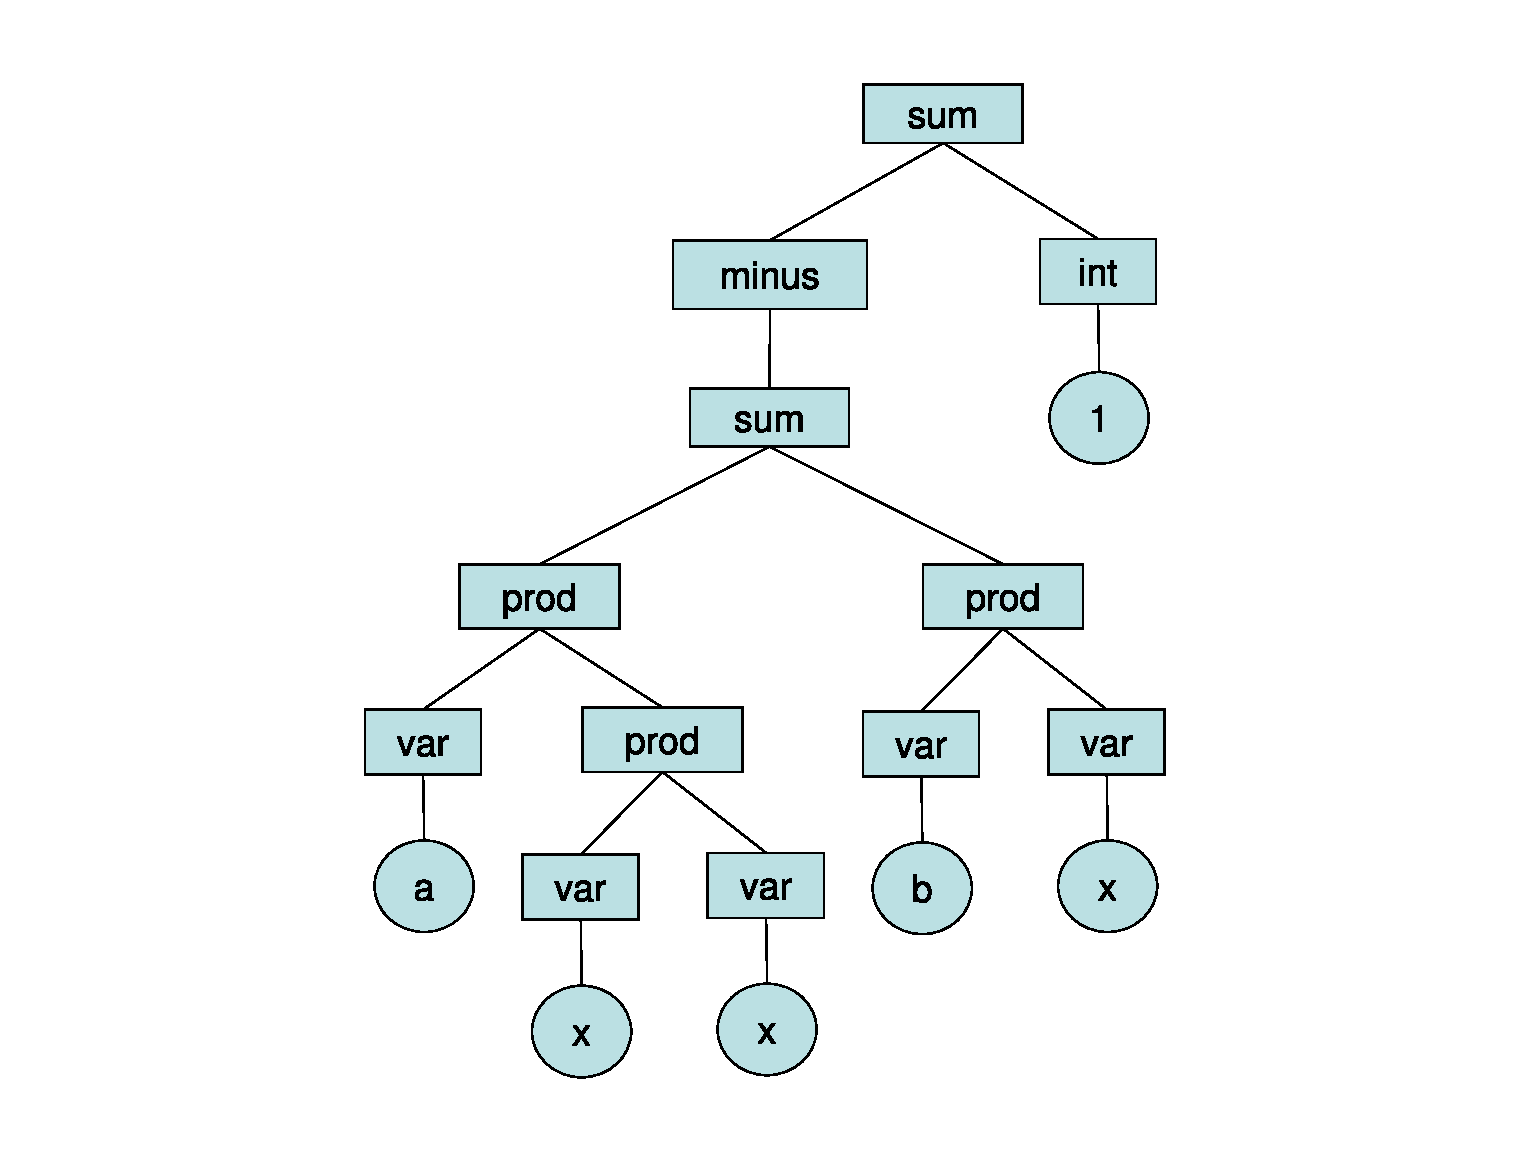
\includegraphics[height=4.5in]{parsetree}
\caption{Parse tree for $-(a(x\cdot x)+ bx) + 1$.}
\label{fig:parse}
\end{figure}

In a computer, such a tree would be represented by pairs or triples
that begin with a
\emph{tag} equal to the label of the top node of the parse tree.  
The general definition of parse trees for $\aexp$'s would be:

\newcommand{\paexp}{\text{Aexp-parse-tree}}

\begin{definition}\label{arithparse}
The set, $\paexp$, of \emph{parse trees for arithmetic expressions} 
over a set of
\emph{variables}, $V$, is defined recursively as follows:
\begin{itemize}
\item \textbf{Base cases:}
\begin{enumerate}
\item If $n \in \integers$, then $\ang{\texttt{int}, n} \in \paexp$.
\item If $v \in V$, then $\ang{\texttt{var}, v} \in \paexp$.
\end{enumerate}
\item \textbf{Constructor cases:} if $e,e' \in \paexp$, then
\begin{enumerate}
\item $\ang{\texttt{sum}, e, e'} \in \paexp$,
\item $\ang{\texttt{prod}, e, e'} \in \paexp$, and
\item $\ang{\texttt{minus}, e} \in \paexp$.
\end{enumerate}
\end{itemize}
\end{definition}

So the $\paexp$ corresponding to formula~\ref{ax} would be:
\begin{equation}\label{axtag}
\begin{array}{rll}
\left< \right. \texttt{sum}, 
         & \left< \right. \texttt{minus},\ \ \left< \right. \texttt{sum},
               & \ang{\texttt{prod},\ \ \ang{\texttt{var},\ a},
                                     \ang{\texttt{prod},\ \
                                            \ang{\texttt{var},\ x},\
                                            \ang{\texttt{var},\ x}}},\\
                               && \left. \left. \ang{\texttt{prod},\ \
                                       \ang{\texttt{var},\ b},\
                                       \ang{\texttt{var},\ x}}
                                   \right> \right>,\\
         & \left. \left. \ang{\texttt{int},\ 1} \right> \right>
\end{array}
\end{equation}
Now the expression~\ref{ax} is certainly a lot more humanly
intelligible than~\ref{axtag}, but~\ref{axtag} is in the
representation best suited and commonly used in compiling and
processing computer programs.

\end{editingnotes}


\begin{editingnotes}

Turn this into a problem

One precise way to determine if a string is matched is to start with 0 and
read the string from left to right, adding 1 to the count for each left
bracket and subtracting 1 from the count for each right bracket.
For example, here are the counts for the two strings above
\[\begin{array}{rrrrrrrrrrrrr}
& \lefbrk & \rhtbrk & \rhtbrk & \lefbrk & \lefbrk & \lefbrk & \lefbrk &
\lefbrk & \rhtbrk & \rhtbrk & \rhtbrk & \rhtbrk\\
0 & 1 & 0 & -1 & 0 & 1 & 2 & 3 & 4 & 3 & 2 & 1 & 0\\
\\
\\
& \lefbrk & \lefbrk & \lefbrk & \rhtbrk & \rhtbrk & \lefbrk & \rhtbrk &
\rhtbrk & \lefbrk & \rhtbrk\\
0 & 1 & 2 & 3 & 2 & 1 & 2 & 1 & 0 & 1 & 0
\end{array}\]
A string has a \term{good count} if its running count never goes
negative and ends with 0.  So the second string above has a good count, but
the first one does not because its count went negative at the third step.
\begin{definition}\label{gc-def}
Let
\[
\GC \eqdef \set{ s \in \brkts \suchthat s\ \text{has a good count}}.
\]
\end{definition}
\end{editingnotes}

\endinput
